\chapter{Grundlagen}

\section{Projektumfeld}

Das Projekt wird im Umfeld der \gls{DHBW} Karlsruhe im Rahmen einer Studienarbeit durchgeführt.
Ziel der Studienarbeit ist es, ein praktisches Projekt zu entwickeln und dies entsprechend zu dokumentieren.
Der Zeitrahmen für dieses Projekt und die Studienarbeit beläuft sich auf ein halbes Jahr.

\section{Funktionsweise \gls{WLAN}} \label{sec:grundlagen-wlan}

Unter \gls{WLAN} versteht man im Allgemeinen ein Funknetz nach einem Standard der \gls{IEEE} 802.11 Familie.
Alle Standards der Familie basieren auf dem ursprünglichen 802.11 Standard und erweitern diesen um neue Funktionalität, Frequenzen und höheren Datenraten.
(vgl. \cite{Schnabel2020})
\TODO{Primärquelle finden}

Für die Funktionsweise des Paper-Trackers muss der Teil der \enquote{Service Sets} der Spezifikation detailiert erleutert werden.
Unter einem Service Set versteht man im Allgemeinen alle Geräte in einem \gls{WLAN}-Netzwerk.
Auf diesen basiert die Lokalisierung der Dokumente.

\subsection{\gls{BSS}}

Ein \gls{BSS} ist Service Set, in dem es nur einen \gls{AP} und damit ein Gerät, dass das Funknetz aufbaut, gibt.
Zu diesem \gls{AP} können beliebig viele Klienten verbunden sein.
In einem solchen Netzwerk besitzt der \gls{AP} eine \gls{SSID} und eine \gls{BSSID}.
Die \gls{SSID} ist der Name des Netzwerks, das von einem Endbenutzer ausgewählt wird, um sich mit dem \gls{WLAN} zu verbinden.
Da mehrere \gls{BSS} die gleiche \gls{SSID} verwenden können, besitzt der \gls{AP} auch eine \gls{BSSID}.
Diese ist meist die \gls{MAC}-Adresse des \gls{AP}, welche per Definition einzigartig ist.
(vgl. \cite{Luber2018})
\TODO{Primärquelle finden (IEEE RFC)}
Mit Hilfe dieser \gls{BSSID} können Klienten zwischen den verschiedenen Netzwerken mit identischer \gls{SSID} unterscheiden.

\subsection{\gls{ESS}}

In einem \gls{ESS} existieren mehrere \gls{BSS}, die miteinander z.B. über ein \gls{LAN} verbunden sind.
Alle \gls{BSS} in diesem Service Set haben eine eigene \gls{BSSID} aber bauen ein Netz mit der gleichen \gls{SSID} auf.
So können Klienten z.B. in größeren Gebäuden zwischen verschiedenen \gls{BSS} wechseln, ohne es zu bemerken.
(vgl. \cite{Haider2019})
\TODO{Primärquelle finden}

\subsection{Signalstärke \gls{RSSI}}

Die \gls{RSSI} ist eine Größe, welche im Allgemeinen die Energie eines Radiosignals repräsentiert.
Es gibt keine Standardisierung hinsichtlich der Messmethode oder der entstehenden Einheit, in
welcher die \gls{RSSI} angegeben wird. Da sie ein Maß für Dämpfung ist, wird jedoch immer eine
negative Zahl angegeben. Je näher sich diese Zahl null nähert, desto stärker ist das Signal.
Typischerweise liegt der Messwert im Bereich zwischen null und $-100$.

Als standardisierter Ersatz für die \gls{RSSI} wurde der \gls{RCPI} eingeführt. Diese Größe wird
immer in der Einheit dBm angegeben und wird über ein definiertes Intervall gemessen. Der
Wertebereich bewegt sich dabei zwischen $-110 dBm$ und $0 dBm$. Repräsentiert wird die Messung als
8-Bit-Ganzzahl, was abzüglich einiger reservierter Werte zu einer maximalen Auflösung von $0.5 dBm$
führt. Auch standardisiert ist die zu erreichende Genauigkeit, so soll die Abweichung bei maximial
$5 dBm$ liegen. (vgl. \cite{IEEE802.11-2012})

\section{Beispiel eines Workflows}

In folgender \autoref{fig:beschaffungsverfahren} ist ein Beispiel für einen Prozess an der \gls{DHBW} Karlsruhe dargestellt.
Es ist das \enquote{Beschaffungs-Genehmigungsverfahren}, das benötigt wird, um eine Bestellung für die \gls{DHBW} durchzuführen.

\begin{figure}[h!tbp]
	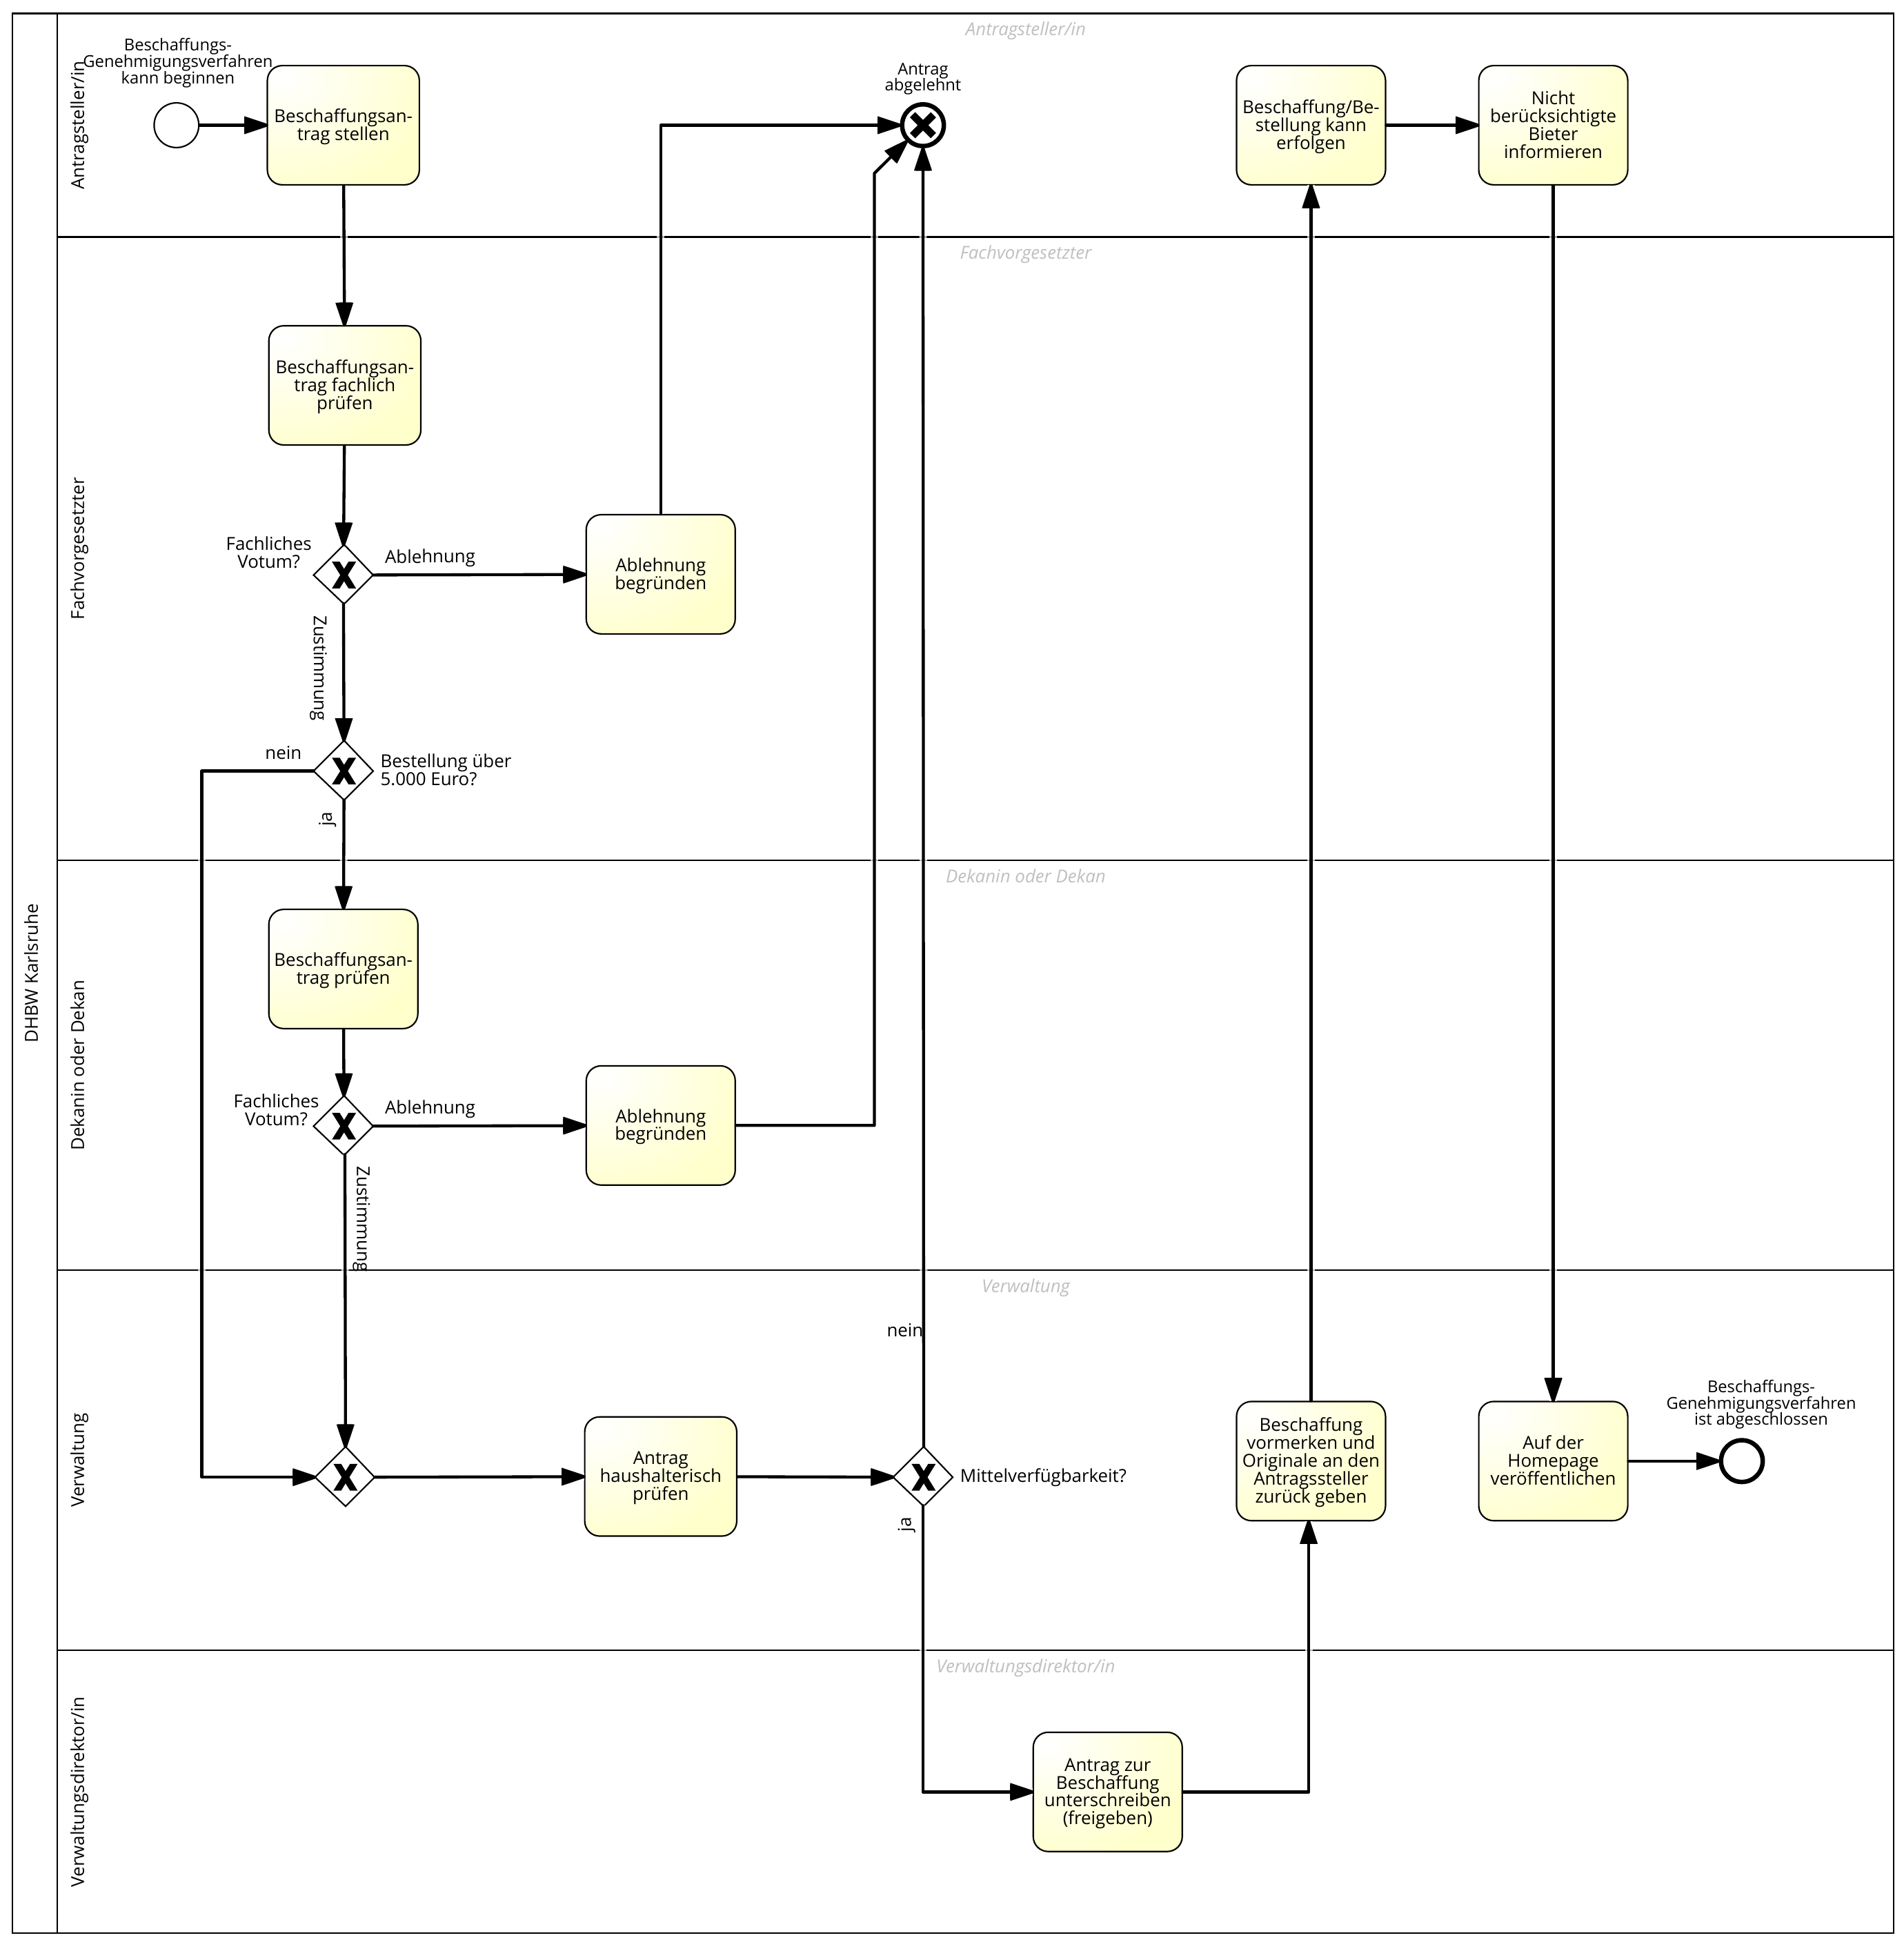
\includegraphics[width=\textwidth]{images/beschaffungs-genehmigungsverfahren.png}
	\centering
	\caption{Beschaffungs-Genehmigungsverfahren der \gls{DHBW}}
	\label{fig:beschaffungsverfahren}
\end{figure}

Der Prozess beginnt mit dem Antragsteller, welcher den Beschaffungsantrag stellt.
Der Antrag geht zum Fachvorgesetzten des Antragsteller, welcher diesen fachlich prüft.
Ist die Prüfung nicht erfolgreich, wird eine Ablehnung begründet und der Prozess beendet.

Bei erfolgreicher Prüfung muss der Antrag, wenn er über 5.000€ liegt, zudem vom Dekan geprüft werden.
Dieser kann entweder den Antrag wie oben beschrieben ablehnen oder stimmt diesem zu.

Ist der Antrag für eine Bestellung unter 5.000€ oder er bekommt die Zustimmung des Dekans, erhält als nächstes die Verwaltung den Antrag.
Die Verwaltung muss prüfen, ob die Mittel für diese Bestellung vorhanden sind.
Sind die Mittel nicht vorhanden, wird der Antrag abgelehnt.
Bei vorhandenen Mitteln wird der Antag von dem Verwaltungsdirektor unterschrieben und damit freigegeben.
Damit wird die Beschaffung in der Verwaltung vorgemerkt und der Antrag geht an den ursprünglichen Antragsteller zurück.

Sobald der Antragsteller den unterzeichneten Antrag erhält, kann die Beschaffung erfolgen.
In diesem Schritt müssen mögliche nicht berücksichtigte Bieter im Falle einer Ausschreibung informiert werden.

Im letzten Schritt veröffentlicht die Verwaltung das Ergebnis der Beschaffung auf der Homepage und der Prozess ist erfolgreich abgeschlossen.
